\documentclass[conference]{IEEEtran}
\usepackage[utf8]{inputenc}
\usepackage{amsmath}
\usepackage{booktabs}
\usepackage{graphicx}
\usepackage{xurl}
\usepackage[hidelinks]{hyperref}

\begin{document}

\title{Traditional Machine Learning versus Deep Learning for Phishing Detection in Remote Work Environments: A Reproducible Comparison of Accuracy, Class Imbalance and Latency}

\author{\IEEEauthorblockN{Altair Tussupov}
\IEEEauthorblockA{Department of Computer Science and Engineering\\
Astana IT University, Astana, Kazakhstan\\
Email: altair.tussupov@gmail.com}}

\maketitle

\begin{abstract}
Published comparisons of machine learning (ML) and deep learning (DL) phishing detectors are rarely comparable: they use different datasets, balanced test sets and, almost never, latency measured on ordinary hardware. We compare seven traditional ML classifiers and four DL models under one protocol on two public datasets: the UCI Phishing Websites dataset (11,055 rows, 30 features) and the Ebbu2017 corpus of raw URLs (54,634 unique URLs after cleaning). All code, data versions and raw results are released. We report four findings. (1) 47.1\% of the UCI rows are exact duplicates; removing them lowers the accuracy of every model, by up to 3.78 percentage points (pp) for a decision tree. (2) On deduplicated feature vectors DL brings no gain: XGBoost reaches 95.50\% accuracy and a 1D-CNN 94.31\%. On raw URL strings a character-level CNN reaches an F1 of 96.84\% against 92.45\% for the best ML model on 20 lexical features. (3) When phishing makes up 1\% of the test traffic, precision falls to 13.3\% for Random Forest and 29.7\% for the CNN, while accuracy stays near 94--98\%, below the 99\% of a trivial ``always legitimate'' rule; the drop matches the analytic prediction within 0.12 pp. (4) On one CPU thread the three character-level DL models, XGBoost, logistic regression and the decision tree classify a URL in under 1~ms (median); the most accurate model is also among the fastest, so the latency--accuracy trade-off assumed in the literature does not appear at this model size.
\end{abstract}

\begin{IEEEkeywords}
Phishing detection, machine learning, deep learning, class imbalance, inference latency, reproducibility, remote work
\end{IEEEkeywords}

% ============================================================================
\section{Introduction}

The shift to remote work in 2020 moved a large share of corporate communication to e-mail and other online channels, used from home networks and personal devices. Attackers reacted quickly: Barracuda reported that COVID-19-themed spear-phishing rose by 667\% between the end of February and March 2020 \cite{barracuda2020}, and a STRIDE risk analysis of social networks motivated by pandemic-era remote work identified phishing as their main threat \cite{sharma2023}.

Three practical properties decide whether a detector is useful in this setting, and published work reports them unevenly.

\emph{Class imbalance.} Phishing is rare in real traffic. Ho et~al. \cite{ho2019} found hundreds of lateral phishing e-mails among 113 million employee-sent e-mails of 92 organizations. Yet most benchmark datasets are close to balanced, and accuracy measured on them says little about precision in deployment.

\emph{Comparability.} Accuracy figures for ML and DL detectors come from different datasets and protocols, so they cannot be put side by side.

\emph{Cost.} Detection on a remote worker's machine must be fast and small, but inference latency on commodity hardware is rarely measured.

This paper addresses these points with experiments rather than with figures collected from different studies. Its contributions are:
\begin{enumerate}
\item A comparison of seven ML and four DL models under one protocol on two public datasets, with accuracy, precision, recall, F1, false-positive rate (FPR), Matthews correlation coefficient (MCC) and PR-AUC.
\item Evidence that duplicate rows in the widely used UCI dataset inflate cross-validated accuracy, with the size of the effect per model.
\item A measurement of how precision collapses at realistic phishing prevalence, and a check that a closed-form expression predicts it.
\item End-to-end CPU latency, model size and memory for every model, and a measured two-tier (fast--slow) cascade.
\item A public repository with code, pinned data versions and the raw predictions behind every table.
\end{enumerate}

Section~\ref{sec:related} reviews related work, Section~\ref{sec:method} describes the methodology, Section~\ref{sec:results} presents the results, Section~\ref{sec:discussion} discusses them together with limitations and open problems, and Section~\ref{sec:conclusion} concludes.

% ============================================================================
\section{Related Work}\label{sec:related}

\emph{Traditional ML on engineered features.} Shahrivari et~al. \cite{shahrivari2020} compared nine classifiers (twelve configurations, counting four SVM kernels) on the UCI Phishing Websites dataset \cite{uci2012}, which holds 6,157 legitimate and 4,898 phishing websites described by 30 features. With 10-fold cross-validation, XGBoost reached 98.32\% accuracy and Random Forest 97.27\%. The features include WHOIS, DNS and page-content attributes, so computing them for a new URL requires network look-ups.

\emph{Deep learning.} Yerima and Alzaylaee \cite{yerima2020} applied a 1D-CNN to the same UCI feature vectors. Their best configuration reached 97.3\% accuracy, 98.2\% recall and an F1 of 0.976 in 10-fold cross-validation, on a 4~GB RAM Linux machine. Sahingoz et~al. \cite{sahingoz2019} built the Ebbu2017 corpus of PhishTank and legitimate URLs and classified URLs from lexical and NLP features.

\emph{Large language models.} Blake \cite{blake2025} fine-tuned Llama-Guard-3-1B with Low-Rank Adaptation (LoRA), which trains only small low-rank matrices added to a frozen model. The resulting Phishsense-1B reached 97.5\% accuracy on a balanced custom e-mail dataset, but 70\% on a harder real-world dataset.

\emph{Datasets and deployment.} The MeAJOR corpus \cite{mendes2025} merges five open sources into 135,894 e-mails; on it XGBoost reached an F1 of 98.34\%, ahead of RF, MLP and CNN baselines. PhishIntel \cite{li2024} addresses latency in deployment with a fast task (local blacklist and result cache) and a slow task (online blacklist, page crawling and a reference-based detector); its authors note that crawling and analysis can each take up to about ten seconds, while users expect a response within about two seconds.

\emph{Gap.} None of these studies compares ML and DL on the same data under realistic prevalence while also measuring latency on commodity hardware. Accuracies from \cite{shahrivari2020,yerima2020,blake2025,mendes2025} come from different datasets and tasks (websites, URLs, e-mails) and are not directly comparable.

% ============================================================================
\section{Methodology}\label{sec:method}

\subsection{Datasets}

\emph{D1 -- UCI Phishing Websites} \cite{uci2012}: 11,055 rows, 30 ternary features, 4,898 phishing (44.3\%) and 6,157 legitimate. We use the copy published with \cite{shahrivari2020}. 5,206 rows (47.1\%) are exact duplicates of other rows, leaving 5,849 unique rows (3,019 phishing, 51.6\%). In 64 cases the same feature vector appears with both labels.

\emph{D2 -- Ebbu2017 URLs} \cite{sahingoz2019}: 37,175 phishing and 36,400 legitimate URLs. In this corpus 36.8\% of legitimate URLs but only 1.8\% of phishing URLs begin with \texttt{https://}, an artefact of how the two classes were collected. We therefore remove the scheme from every URL and then drop duplicate URL strings. This leaves 54,634 unique URLs: 24,726 phishing (45.3\%) and 29,908 legitimate. The median URL length is 49 characters; 5.3\% of URLs exceed 128 characters.

Both datasets are fetched from pinned commits and verified by SHA-256 checksums (Section~\ref{sec:repro}).

\subsection{Models}

\emph{Traditional ML (7 models)}, scikit-learn and XGBoost with fixed hyper-parameters (no tuning): logistic regression; decision tree; Random Forest (300 trees); AdaBoost (200 estimators); SVM with RBF kernel ($C{=}1$, $\gamma$=\texttt{scale}); KNN ($k{=}5$); XGBoost (300 trees, depth 6, learning rate 0.1). Logistic regression, SVM and KNN receive standardized inputs.

On D1 these models use the 30 dataset features. On D2 they use 20 lexical features computed from the URL string alone, without network access: lengths of URL, host and path; counts of dots, hyphens, digits, slashes, \texttt{@}, \texttt{?}, \texttt{=}, \texttt{\_} and \texttt{\%}; number of subdomains; IP-address host; \texttt{www} prefix; digit ratio; Shannon entropy; number of suspicious keywords; top-level-domain length; longest token.

\emph{Deep learning (4 models)}, PyTorch on CPU:
\begin{itemize}
\item \textbf{1D-CNN on D1}, re-implementing the best configuration of \cite{yerima2020}: two convolution blocks (64 filters of length 12 and 6, max-pooling 2), a 32-unit dense layer, sigmoid output; 41,921 parameters.
\item \textbf{CNN (char)} on D2: 32-dimensional character embedding, three parallel convolutions (kernels 3, 5, 7; 64 filters each), global max-pooling, a 64-unit dense layer; 46,433 parameters.
\item \textbf{LSTM (char)} on D2: the same embedding, one LSTM layer with 64 units; 28,257 parameters.
\item \textbf{CNN+LSTM (char)} on D2: embedding, a convolution (64 filters, kernel 5), max-pooling 2, an LSTM layer with 64 units; 46,753 parameters.
\end{itemize}
URLs are encoded as printable-ASCII codes and truncated or padded to 128 characters. All DL models use Adam (learning rate $10^{-3}$) and binary cross-entropy. The weights with the lowest validation loss are kept. On D2: batch 128, at most 10 epochs, patience 2. On D1: batch 64, at most 200 epochs, patience 20, following \cite{yerima2020}.

\subsection{Evaluation protocols}

\emph{D1.} Stratified 10-fold cross-validation (seed 42) under two protocols. Protocol~A uses all 11,055 rows, as in \cite{shahrivari2020}. Protocol~B uses the 5,849 unique rows, so no feature vector appears in both training and test folds. The 1D-CNN holds out 10\% of each training fold for early stopping.

\emph{D2.} Stratified 80/20 train/test split, repeated with seeds 42, 43 and 44 (10,927 test URLs per seed). ML models are fitted on the training part. DL models hold out 10\% of the training part for early stopping. The test part is never used for training, tuning or early stopping. We report mean $\pm$ standard deviation over seeds.

\emph{Prevalence.} To measure the effect of class imbalance, we keep all legitimate test URLs of D2 and randomly draw phishing test URLs so that phishing makes up 10\%, 2\% or 1\% of the test set (50 draws per level and seed). The trained models and the 0.5 decision threshold (0 for the SVM decision value) are not changed.

\subsection{Metrics}

The positive class is phishing. Besides accuracy, precision, recall and F1 we report FPR, MCC and the area under the precision--recall curve (PR-AUC), which remain informative under imbalance. For a classifier with true-positive rate TPR and false-positive rate FPR, precision at phishing prevalence $\pi$ is
\begin{equation}
\text{Precision}(\pi) = \frac{\text{TPR}\cdot\pi}{\text{TPR}\cdot\pi + \text{FPR}\cdot(1-\pi)}.
\label{eq:precision}
\end{equation}
We compare this prediction, computed from each model's TPR and FPR on the full test set, with the measured precision.

\emph{Latency and memory.} Each fitted seed-42 D2 model is loaded in a fresh process limited to one CPU thread. We time the end-to-end path from raw URL string to probability (feature extraction or character encoding included) for 1,000 test URLs, one at a time, after 50 warm-up calls, and report the median and 95th percentile. We also report the time per URL when the same 1,000 URLs are classified in one batch, the size of the serialized model file, and the increase of the process's peak resident memory over its value after loading the libraries. D1 latency is not reported because its features require network look-ups that dominate the cost.

\subsection{Hardware and software}

All experiments ran on one virtual machine: Intel Xeon processor at 2.80~GHz (2 logical CPUs), 7.8~GB RAM, no GPU, Linux kernel 6.18, Python 3.13.16, NumPy 2.5.3, pandas 3.0.5, scikit-learn 1.9.1, XGBoost 3.4.1 and PyTorch 2.14.1 (CPU execution). Training used two threads. For seed 42 another experiment shared the CPU, so training times are averaged over seeds 43 and 44 only.

\subsection{Reproducibility}\label{sec:repro}

The repository [\emph{URL to be added}] contains the code of every experiment, a script that downloads the datasets from pinned commits and checks their SHA-256 sums, the per-fold and per-seed results, the test-set predictions of every model and the script that generates every table of this paper from those files. A single command re-runs all experiments.

% ============================================================================
\section{Results}\label{sec:results}

\subsection{Duplicates inflate accuracy on the UCI dataset}

Table~\ref{tab:uci} shows that under Protocol~A our results reproduce those of \cite{shahrivari2020} closely: Random Forest reaches 97.25\% (97.27\% in \cite{shahrivari2020}). XGBoost reaches 97.11\% (98.32\% in \cite{shahrivari2020}, where it was tuned), and the 1D-CNN 96.13\% (97.3\% in \cite{yerima2020}).

Removing duplicates (Protocol~B) lowers the accuracy of every model. Models that memorise individual examples lose most: the decision tree loses 3.78~pp, Random Forest 2.40~pp and KNN 2.17~pp. Under Protocol~B XGBoost is the most accurate model (95.50\%), and the 1D-CNN (94.31\%) does not outperform the tree ensembles. With 47\% duplicated rows, part of the accuracy reported on this dataset reflects examples seen during training.

% generated by src/make_tables.py from results/*.csv -- do not edit by hand
\begin{table*}[t]
\centering
\caption{UCI Phishing Websites, 10-fold CV. A: all 11,055 rows (protocol of [3]); B: 5,849 unique rows. Mean $\pm$ std over folds.}
\label{tab:uci}
\resizebox{\textwidth}{!}{%
\begin{tabular}{lrrrrrr}
\toprule
Model & Acc. A (\%) & Acc. B (\%) & $\Delta$ (pp) & F1 B (\%) & MCC B & Train B (s) \\
\midrule
Logistic Regression & 92.72 $\pm$ 0.64 & 92.02 $\pm$ 1.07 & -0.70 & 92.21 & 0.840 & 0.11 \\
Decision Tree & 96.39 $\pm$ 0.50 & 92.61 $\pm$ 0.88 & -3.78 & 92.89 & 0.852 & 0.01 \\
Random Forest & 97.25 $\pm$ 0.37 & 94.85 $\pm$ 0.88 & -2.40 & 94.98 & 0.897 & 1.24 \\
AdaBoost & 93.47 $\pm$ 0.56 & 93.40 $\pm$ 0.92 & -0.07 & 93.52 & 0.868 & 1.04 \\
SVM (RBF) & 95.37 $\pm$ 0.44 & 94.32 $\pm$ 0.82 & -1.05 & 94.47 & 0.887 & 3.36 \\
KNN (k=5) & 94.64 $\pm$ 0.58 & 92.48 $\pm$ 0.96 & -2.17 & 92.79 & 0.850 & 0.01 \\
XGBoost & 97.11 $\pm$ 0.28 & 95.50 $\pm$ 0.69 & -1.60 & 95.64 & 0.910 & 0.31 \\
1D-CNN [7] & 96.13 $\pm$ 0.44 & 94.31 $\pm$ 1.02 & -1.82 & 94.47 & 0.886 & 37.06 \\
\bottomrule
\end{tabular}
}
\end{table*}


\subsection{Raw URLs: character-level DL outperforms lexical-feature ML}

On D2 the ranking reverses (Table~\ref{tab:urls}). All three character-level models outperform all seven ML models. CNN (char) reaches an F1 of 96.84\% with an FPR of 2.40\%, against 92.45\% and 6.05\% for the best ML model (Random Forest), so the CNN produces 2.5 times fewer false alarms. The variation across seeds is small (standard deviation of F1 at most 0.89~pp, and at most 0.43~pp for the DL models). The hybrid CNN+LSTM does not improve on the plain CNN.

The advantage comes from the input representation, not from depth alone. With 20 hand-crafted lexical features the ML models lose information that the character models learn directly. On D1, where both families see the same 30 features, DL has no advantage.

% generated by src/make_tables.py from results/*.csv -- do not edit by hand
\begin{table*}[t]
\centering
\caption{Ebbu2017 URLs (54,634 unique), stratified 80/20 split, mean $\pm$ std over 3 seeds. ML: 20 lexical features; DL: raw characters.}
\label{tab:urls}
\resizebox{\textwidth}{!}{%
\begin{tabular}{lrrrrrrrr}
\toprule
Model & Type & Acc. (\%) & Prec. (\%) & Rec. (\%) & F1 (\%) & FPR (\%) & PR-AUC & Train (s) \\
\midrule
Logistic Regression & ML & 85.82 $\pm$ 0.45 & 85.70 & 82.41 & 84.02 $\pm$ 0.57 & 11.37 & 0.9253 & 0.4 \\
Decision Tree & ML & 89.77 $\pm$ 0.48 & 88.70 & 88.70 & 88.70 $\pm$ 0.54 & 9.34 & 0.8395 & 0.3 \\
Random Forest & ML & 93.18 $\pm$ 0.16 & 92.66 & 92.25 & 92.45 $\pm$ 0.16 & 6.05 & 0.9761 & 8.6 \\
AdaBoost & ML & 87.18 $\pm$ 0.71 & 86.72 & 84.64 & 85.67 $\pm$ 0.89 & 10.72 & 0.9412 & 6.9 \\
SVM (RBF) & ML & 91.32 $\pm$ 0.20 & 91.17 & 89.50 & 90.33 $\pm$ 0.23 & 7.17 & 0.9624 & 32.0 \\
KNN (k=5) & ML & 91.67 $\pm$ 0.14 & 90.36 & 91.33 & 90.84 $\pm$ 0.16 & 8.06 & 0.9384 & 0.0 \\
XGBoost & ML & 93.04 $\pm$ 0.26 & 92.63 & 91.94 & 92.28 $\pm$ 0.28 & 6.05 & 0.9777 & 1.0 \\
CNN (char) & DL & 97.15 $\pm$ 0.08 & 97.10 & 96.60 & 96.84 $\pm$ 0.08 & 2.40 & 0.9957 & 175.8 \\
LSTM (char) & DL & 95.87 $\pm$ 0.39 & 95.67 & 95.18 & 95.42 $\pm$ 0.43 & 3.57 & 0.9907 & 626.7 \\
CNN+LSTM (char) & DL & 96.60 $\pm$ 0.29 & 96.98 & 95.48 & 96.22 $\pm$ 0.35 & 2.46 & 0.9940 & 296.5 \\
\bottomrule
\end{tabular}
}
\end{table*}


\subsection{Precision collapses at realistic prevalence}

Table~\ref{tab:imbalance} and Fig.~\ref{fig:prevalence} evaluate the same trained models at decreasing phishing prevalence. Recall and FPR do not depend on prevalence and stay constant, but precision falls sharply. At 1\% phishing, precision is 13.34\% for Random Forest and 13.22\% for XGBoost: about seven of every eight alerts are false. For CNN (char) it is 29.66\%. Accuracy stays near 94\% for the ML models and 97.6\% for the CNN, below the 99\% that a trivial ``always legitimate'' rule would score; accuracy is therefore not a meaningful metric at this prevalence. MCC and PR-AUC separate the models better: at 1\% phishing, PR-AUC is 0.58 for Random Forest and 0.90 for the CNN.

Across all ten models and four prevalence levels, Eq.~\eqref{eq:precision} predicts the measured precision within 0.12~pp. Precision at a target prevalence can therefore be estimated from TPR and FPR measured on a balanced test set, without collecting an imbalanced one. Because precision at low prevalence is governed by FPR, the 2.5-fold lower FPR of the CNN translates into more than twice the precision of the ML models.

\begin{figure}[t]
\centering
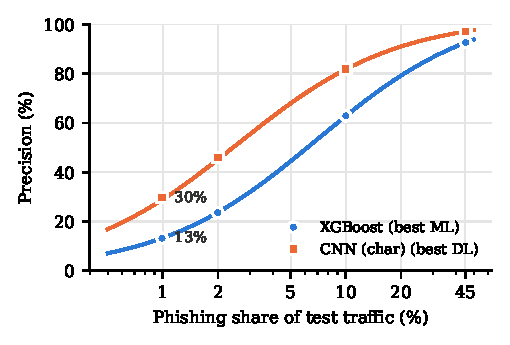
\includegraphics[width=\columnwidth]{fig_precision_prevalence.pdf}
\caption{Precision versus phishing share of the test set. Markers: measured (mean over 50 draws and three seeds); lines: Eq.~\eqref{eq:precision} with each model's TPR and FPR on the full test set.}
\label{fig:prevalence}
\end{figure}

% generated by src/make_tables.py from results/*.csv -- do not edit by hand
\begin{table*}[t]
\centering
\caption{Same models at lower phishing prevalence (all legitimate test URLs kept, phishing sub-sampled; mean of 50 draws $\times$ seeds). Threshold fixed at 0.5.}
\label{tab:imbalance}
\resizebox{\textwidth}{!}{%
\begin{tabular}{lrrrrrrrr}
\toprule
Model & Phishing share & Acc. (\%) & Prec. (\%) & Prec. formula (\%) & Rec. (\%) & F1 (\%) & MCC & PR-AUC \\
\midrule
Random Forest & 45.2\% & 93.18 & 92.66 & 92.66 & 92.25 & 92.45 & 0.862 & 0.976 \\
Random Forest & 10.0\% & 93.80 & 62.96 & 62.93 & 92.37 & 74.87 & 0.732 & 0.885 \\
Random Forest & 2.0\% & 93.92 & 23.73 & 23.76 & 92.10 & 37.73 & 0.450 & 0.684 \\
Random Forest & 1.0\% & 93.94 & 13.34 & 13.29 & 92.62 & 23.31 & 0.339 & 0.577 \\
XGBoost & 45.2\% & 93.04 & 92.63 & 92.63 & 91.94 & 92.28 & 0.860 & 0.978 \\
XGBoost & 10.0\% & 93.75 & 62.85 & 62.84 & 92.00 & 74.67 & 0.729 & 0.896 \\
XGBoost & 2.0\% & 93.90 & 23.63 & 23.70 & 91.58 & 37.55 & 0.448 & 0.734 \\
XGBoost & 1.0\% & 93.93 & 13.22 & 13.26 & 91.69 & 23.10 & 0.335 & 0.660 \\
CNN (char) & 45.2\% & 97.15 & 97.10 & 97.10 & 96.60 & 96.84 & 0.943 & 0.996 \\
CNN (char) & 10.0\% & 97.50 & 81.93 & 81.93 & 96.61 & 88.61 & 0.876 & 0.977 \\
CNN (char) & 2.0\% & 97.58 & 45.93 & 45.95 & 96.53 & 61.97 & 0.656 & 0.930 \\
CNN (char) & 1.0\% & 97.59 & 29.66 & 29.69 & 96.46 & 45.10 & 0.526 & 0.901 \\
CNN+LSTM (char) & 45.2\% & 96.60 & 96.98 & 96.98 & 95.48 & 96.22 & 0.932 & 0.994 \\
CNN+LSTM (char) & 10.0\% & 97.33 & 81.19 & 81.19 & 95.49 & 87.75 & 0.866 & 0.969 \\
CNN+LSTM (char) & 2.0\% & 97.49 & 44.14 & 44.24 & 95.13 & 60.27 & 0.639 & 0.901 \\
CNN+LSTM (char) & 1.0\% & 97.51 & 28.03 & 28.08 & 95.23 & 43.29 & 0.509 & 0.862 \\
\bottomrule
\end{tabular}
}
\end{table*}


\subsection{Latency, model size and memory}

Table~\ref{tab:latency} shows that on one CPU thread XGBoost classifies a URL in a median 0.48~ms and CNN (char) in 0.50~ms, feature extraction and encoding included. The recurrent models are slower but still under 1~ms (median) and under 1.7~ms (95th percentile). The slowest models are the scikit-learn ensembles: Random Forest (23.6~ms) and AdaBoost (31.2~ms) pay a fixed per-call cost for evaluating hundreds of estimators on a single sample. When URLs are classified in batches, every model needs less than 1~ms per URL.

The character models are small: 0.11--0.18~MB on disk, against 191.9~MB for the 300-tree Random Forest. Their peak memory increase of 125--155~MB is dominated by the PyTorch runtime rather than by the weights.

As an illustration, 10,000 employees receiving 50 e-mails a day with one URL each produce 500,000 URLs a day. At 0.50~ms per URL the CNN needs about 250~s of CPU time a day for this load.

% generated by src/make_tables.py from results/*.csv -- do not edit by hand
\begin{table*}[t]
\centering
\caption{End-to-end single-URL inference on CPU (1 thread, batch 1, 1,000 URLs after 50 warm-up calls), model size on disk and peak RSS increment.}
\label{tab:latency}
\resizebox{\textwidth}{!}{%
\begin{tabular}{lrrrrrr}
\toprule
Model & F1 (\%) & Median (ms) & p95 (ms) & Batched (ms/URL) & Size (MB) & RAM incr. (MB) \\
\midrule
Logistic Regression & 84.02 & 0.461 & 0.941 & 0.030 & 0.002 & 8.0 \\
Decision Tree & 88.70 & 0.165 & 0.445 & 0.051 & 0.609 & 8.9 \\
Random Forest & 92.45 & 23.599 & 36.680 & 0.183 & 191.907 & 391.2 \\
AdaBoost & 85.67 & 31.153 & 51.315 & 0.067 & 0.123 & 8.9 \\
SVM (RBF) & 90.33 & 1.393 & 2.226 & 0.802 & 1.918 & 8.9 \\
KNN (k=5) & 90.84 & 4.263 & 6.614 & 0.296 & 3.670 & 10.2 \\
XGBoost & 92.28 & 0.478 & 0.714 & 0.046 & 0.921 & 14.5 \\
CNN (char) & 96.84 & 0.502 & 0.825 & 0.412 & 0.181 & 154.5 \\
LSTM (char) & 95.42 & 0.797 & 1.658 & 0.221 & 0.111 & 140.7 \\
CNN+LSTM (char) & 96.22 & 0.972 & 1.682 & 0.276 & 0.182 & 124.6 \\
\bottomrule
\end{tabular}
}
\end{table*}


\subsection{A two-tier cascade}

The cascade in Table~\ref{tab:cascade} sends a URL to CNN (char) only when the XGBoost probability is uncertain ($|p-0.5|<\delta$). Escalating 8.5\% of URLs ($\delta=0.2$) raises F1 from 92.28\% to 95.10\%; escalating 24.4\% ($\delta=0.4$) gives 96.57\%, close to the CNN alone (96.84\%). Here the cascade brings no saving, because the CNN is about as fast as XGBoost. A fast--slow design pays off only when the second tier is much more expensive than the first, as with the page crawling and reference-based analysis of PhishIntel \cite{li2024}, which take seconds. In that case the mean cost per URL is $t_1 + r\,t_2$, where $r$ is the escalation rate measured here.

% generated by src/make_tables.py from results/*.csv -- do not edit by hand
\begin{table}[t]
\centering
\caption{Two-tier cascade: XGBoost, escalating to CNN (char) when $|p-0.5|<\delta$ ($\delta$=0: XGBoost only; 0.5: DL only).}
\label{tab:cascade}
\resizebox{\columnwidth}{!}{%
\begin{tabular}{lrrrrr}
\toprule
$\delta$ & Escalated (\%) & Acc. (\%) & F1 (\%) & FPR (\%) & Mean latency (ms) \\
\midrule
0.0 & 0.00 & 93.04 & 92.28 & 6.05 & 0.478 \\
0.1 & 3.99 & 94.38 & 93.77 & 4.85 & 0.498 \\
0.2 & 8.50 & 95.57 & 95.10 & 3.91 & 0.520 \\
0.3 & 14.09 & 96.31 & 95.92 & 3.18 & 0.549 \\
0.4 & 24.35 & 96.90 & 96.57 & 2.72 & 0.600 \\
0.5 & 100.00 & 97.15 & 96.84 & 2.40 & 0.502 \\
\bottomrule
\end{tabular}
}
\end{table}


% ============================================================================
\section{Discussion}\label{sec:discussion}

\subsection{Challenges revisited}

\emph{Class imbalance} is the most serious practical problem we measured. A detector with 97\% accuracy on a balanced test set produces mostly false alarms at 1\% prevalence. Studies should report precision, FPR and PR-AUC at a stated prevalence, or report TPR and FPR so that Eq.~\eqref{eq:precision} can be applied. Deployments should choose the decision threshold for the expected prevalence and an acceptable alert rate.

\emph{Feature engineering versus end-to-end learning.} On a fixed set of engineered features (D1), DL did not beat gradient-boosted trees. On raw URL strings (D2), character models clearly beat 20 lexical features. The choice depends on the input, not on a general superiority of either family.

\emph{The latency--accuracy trade-off} was not observed at the model sizes used here: the most accurate model was also among the fastest. Latency matters mainly for models that need network access (WHOIS, page crawling) or that are large (LLMs).

\emph{Endpoint cost.} Character-level models under 0.2~MB that classify a URL in under a millisecond on one CPU thread are suitable for laptops of remote workers.

\emph{Privacy.} URL-only models run locally and do not need the e-mail body to leave the device. We did not evaluate privacy-preserving training.

\subsection{Limitations}

All experiments ran on one 2-vCPU virtual machine; absolute latencies will differ on other hardware, but the ranking is likely to hold. Ebbu2017 dates from 2017. Despite removing the scheme, other collection artefacts may remain: for example, 58.8\% of legitimate but 26.2\% of phishing URLs start with \texttt{www.}. We evaluate URLs only, not e-mail bodies or attachments, and we did not tune hyper-parameters, so absolute scores are below tuned results in the literature. Imbalanced test sets were built by subsampling phishing URLs, which assumes the legitimate test URLs are representative of real traffic. Three seeds give a limited estimate of variance.

\subsection{Future directions}

\begin{enumerate}
\item \textbf{Prevalence-aware evaluation and thresholds}: calibrate scores and select thresholds for a target alert budget at realistic prevalence.
\item \textbf{E-mail and multi-channel data}: repeat the comparison on e-mail corpora such as MeAJOR \cite{mendes2025} and on chat and collaboration messages used in remote work.
\item \textbf{Federated learning} \cite{mcmahan2017}: train across organizations without sharing e-mails, including the non-IID case where different organizations face different campaigns.
\item \textbf{Explainability}: attribution methods such as SHAP \cite{lundberg2017} to show users why a URL was flagged; their effect on user behaviour needs to be measured.
\item \textbf{Robustness over time}: train on older and test on newer phishing campaigns to measure drift.
\end{enumerate}

% ============================================================================
\section{Conclusion}\label{sec:conclusion}

Under one protocol on two public datasets, we found that: duplicate rows inflate accuracy on the widely used UCI dataset by up to 3.78~pp; DL does not beat gradient-boosted trees on engineered features but outperforms lexical-feature ML on raw URLs (F1 96.84\% versus 92.45\%); at 1\% phishing prevalence precision drops to 13--30\% even for the best models, as predicted by a simple closed-form expression; and small character-level models classify a URL in under 1~ms on one CPU thread. Reporting prevalence-aware metrics and measured latency would make future comparisons of phishing detectors more useful for deployment.

\section*{Acknowledgment}
The author thanks the supervisor for feedback on an earlier draft. % Add a disclosure of AI assistance here if required by the venue or university policy.

\begin{thebibliography}{12}

\bibitem{barracuda2020}
Barracuda Networks, ``Threat Spotlight: Coronavirus-related phishing,'' Barracuda Blog, Mar. 26, 2020. [Online]. Available: \url{https://blog.barracuda.com/2020/03/26/threat-spotlight-coronavirus-related-phishing}

\bibitem{sharma2023}
K.~R. Sharma, W.-Y. Chiu, and W.~Meng, ``Security analysis on social media networks via STRIDE model,'' arXiv:2303.13075, 2023.

\bibitem{ho2019}
G.~Ho, A.~Cidon, L.~Gavish, M.~Schweighauser, V.~Paxson, S.~Savage, G.~M. Voelker, and D.~Wagner, ``Detecting and characterizing lateral phishing at scale,'' arXiv:1910.00790, 2019.

\bibitem{shahrivari2020}
V.~Shahrivari, M.~M. Darabi, and M.~Izadi, ``Phishing detection using machine learning techniques,'' arXiv:2009.11116, 2020.

\bibitem{uci2012}
R.~Mohammad and L.~McCluskey, ``Phishing Websites,'' UCI Machine Learning Repository, 2012, doi: 10.24432/C51W2X.

\bibitem{yerima2020}
S.~Y. Yerima and M.~K. Alzaylaee, ``High accuracy phishing detection based on convolutional neural networks,'' arXiv:2004.03960, 2020.

\bibitem{sahingoz2019}
O.~K. Sahingoz, E.~Buber, O.~Demir, and B.~Diri, ``Machine learning based phishing detection from URLs,'' \emph{Expert Systems with Applications}, vol.~117, pp.~345--357, 2019, doi: 10.1016/j.eswa.2018.09.029.

\bibitem{blake2025}
S.~E. Blake, ``Phishsense-1B: A technical perspective on an AI-powered phishing detection model,'' arXiv:2503.10944, 2025.

\bibitem{mendes2025}
P.~Mendes, E.~Maia, and I.~Pra\c{c}a, ``MeAJOR Corpus: A multi-source dataset for phishing email detection,'' arXiv:2507.17978, 2025.

\bibitem{li2024}
Y.~Li \emph{et~al.}, ``PhishIntel: Toward practical deployment of reference-based phishing detection,'' in \emph{Companion Proc. ACM Web Conf. (WWW Companion '25)}, 2025, doi: 10.1145/3701716.3715192.

\bibitem{mcmahan2017}
B.~McMahan, E.~Moore, D.~Ramage, S.~Hampson, and B.~A. y~Arcas, ``Communication-efficient learning of deep networks from decentralized data,'' in \emph{Proc. AISTATS}, 2017, pp.~1273--1282.

\bibitem{lundberg2017}
S.~M. Lundberg and S.-I. Lee, ``A unified approach to interpreting model predictions,'' in \emph{Advances in Neural Information Processing Systems 30 (NeurIPS)}, 2017.

\end{thebibliography}

\end{document}
